\documentclass{sig-alternate}

\usepackage{amsmath}
%\usepackage{fullpage}
%\usepackage{doublespace}
\usepackage{epsfig}
\usepackage{subfigure}

\begin{document}

\toappear{
\raisebox{2pt}[2pt]{\underline{~~~~~~~~~~~~~~~~~~~~~~~~~~~~~~~~~~~~~~~~~~~~~~~~~~}} \\
$^*$ This version of the paper is dated August 9, 2002 and
corrects some typos in the ASPLOS final copy.  More information on the
StreamIt project is available from
\texttt{http://compiler.lcs.mit.edu/streamit} \\
~ \\
\small{
Permission to make digital or hard copies of all or part of this work
for personal or classroom use is granted without fee provided that
copies are not made or distributed for profit or commercial advantage
and that copies bear this notice and the full citation on the first
page.  To copy otherwise, to republish, to post on servers or to
redistribute to lists, requires prior specific permission and/or a
fee. \par
{\it ASPLOS X} 10/02 San Jose, CA, USA \par
Copyright 2002 ACM 1-58113-574-2/02/0010 ...\$5.00 \\ ~ \\ ~ \\
}}

\conferenceinfo{ASPLOS X}{10/02 San Jose, CA, USA} 
\CopyrightYear{2002}
\crdata{1-58113-574-2/02/0010}

\title{A Stream Compiler for \\ Communication-Exposed Architectures}

\numberofauthors{1}

\author{Michael I. Gordon, William Thies, Michal Karczmarek, Jasper Lin, Ali S. Meli,\\ Andrew A. Lamb, Chris Leger, Jeremy Wong, Henry Hoffmann,\\ David Maze, and Saman Amarasinghe \\ ~ \\
  MIT Laboratory for Computer Science \\
  200 Technology Square \\
  Cambridge, MA  02139 \\ ~ \\
  \sffamily{\{mgordon, thies, karczma, jasperln, saadat, aalamb, clleger, jnwong, hank, dmaze, saman\}@lcs.mit.edu}}

%previous author format
%only first three authors
%\author{
%\alignauthor Michael I. Gordon\\
%	\affaddr{MIT Laboratory for Computer Science}\\
%	\affaddr{200 Technology Square} \\
%	\affaddr{Cambridge, MA 02139}\\
%	\email{mgordon@cag.lcs.mit.edu}
%\alignauthor William Thies\\
%	\affaddr{MIT Laboratory for Computer Science}\\
%	\affaddr{200 Technology Square} \\
%	\affaddr{Cambridge, MA 02139}\\
%	\email{thies@lcs.mit.edu}
%\alignauthor Michal Karczmarek\\
%	\affaddr{MIT Laboratory for Computer Science}\\
%	\affaddr{200 Technology Square} \\
%	\affaddr{Cambridge, MA 02139}\\
%	\email{karczma@lcs.mit.edu}
%}

%\additionalauthors{Additional Authors: Jeremy Wong, Henry Hoffman, David 
%Maze, and Saman Amarasinghe, email: {\texttt{\{jnwong, hank, dmaze, saman\}@lcs.mit.edu}}}

\date{}

% this is the line spacing
%\setstretch{1.25}

% \sloppy lets Latex be a little less anal about interword spacing.  It is
% one way to eliminate those annoying Overfull hbox warnings.
% Another way is to surround each offending paragraph with
% \begin{sloppypar} ... \end{sloppypar}

%\sloppy

% See page 90 of the Latex book for info about vertical spacing probs.

  \newcommand{\mt}[1]{\mbox{\it #1}}
  \newcommand{\todo}[1]{\framebox{#1}}
  \newcommand{\Radar}[0]{Radar}
  \newcommand{\bibfont}{\fontencoding{OT1}\fontfamily{ptmr}\fontseries{m}
    \fontshape{n} \fontsize{9pt}{12pt}\selectfont}
  \newcommand{\bibfontt}{\fontsize{8pt}{10pt}\selectfont}

  %\toappear{\centerline{\Large\bf MIT LCS Technical Memo,}
  %          \centerline{\Large\bf MIT-LCS-TM-6XX,}
  %          \centerline{\Large\bf November, 2001.}}
  
  \maketitle
  As DSP programming is becoming more complex, there is an increasing
need for high-level abstractions that can be efficiently compiled.
Toward this end, we present a set of aggressive optimizations that
target linear sections of a stream program.  Our input language is
StreamIt, which represents programs as a hierarchical graph of
autonomous filters.  A filter is linear if each of its outputs can be
represented as an affine combination of its inputs.  Linear filters
are common in DSP applications; examples include FIR filters,
expanders, compressors, FFTs and DCTs.

We present a linear extraction analysis that automatically detects
linear filters based on the C-like code in their {\tt work} function.
Once linear filters are identified, we show how neighboring nodes can
be collapsed into a single linear representation, thereby eliminating
many redundant computations.  Also, we describe a method for
automatically translating linear nodes into the frequency domain,
thereby yielding algorithmic savings for convolutional filters.

We have completed a fully-automatic implementation of the above
techniques as part of the StreamIt compiler, and we demonstrate
performance improvements that average 400\% over our benchmark
applications.




  
  %\advance\topmargin by -0.35inn      % Correct for LaTeX gratuitousnes
  %\category{Zah?}{Something else}
  %\terms{Stuff}
  %\keywords{Streams, Raw, Streams}

  \section{Introduction}

Applications that are structured around some notion of a ``stream''
are becoming increasingly important and widespread.  There is evidence
that streaming media applications are already consuming most of the
cycles on consumer machines \cite{Rix98}, and their use is continuing
to grow.  In the embedded domain, applications for hand-held
computers, cell phones, and DSP's are centered around a stream of
voice or video data.  The stream abstraction is also fundamental to
high-performance applications such as intelligent software routers,
cell phone base stations, and HDTV editing consoles.

Despite the prevalence of these applications, there is surprisingly
little language and compiler support for practical, large-scale stream
programming.  Of course, the notion of a stream as a programming
abstraction has been around for decades \cite{SICP}, and a number of
special-purpose stream languages have been designed (see
\cite{survey97} for a review).  Many of these languages and
representations are elegant and theoretically sound, but they often
lack features and are too inflexible to support straightforward
development of modern stream applications, or their implementations
are too inefficient to use in practice.  Consequently, most
programmers turn to general-purpose languages such as C or C++ to
implement stream programs.

There are two reasons that general-purpose languages are inadequate for
stream programming.  Firstly, they are a mismatch for the application
domain.  That is, they do not provide a natural or intuitive
representation of streams, thereby having a negative effect on
readability, robustness, and programmer productivity.  Moreover, because
the widespread parallelism and regular communication patterns of data
streams are left implicit in general-purpose languages, compilers are
not stream-conscious and do not perform stream-specific optimizations.
As a result, performance-critical loops are often hand-coded in a
low-level assembly language and must be re-implemented for each target
architecture.  This practice is labor-intensive, error-prone, and very
costly.

Secondly, general-purpose languages are a mismatch for the emerging
class of grid-based architectures \cite{smartmemories,rawshort,trips} that
are especially well-suited for stream processing.  Perhaps the primary
appeal of C is that it provides a ``common machine language'' for
von-Neumann architectures.  That is, it abstracts away the
idiosyncratic differences between machines, but encapsulates their
common properties: a single program counter, arithmetic operations,
and a monolithic memory.  However, for grid-based architectures, the
von-Neumann model no longer holds, as there are multiple instruction
streams and distributed memory banks.  Thus, C no longer serves as a
common machine language--in fact, it provides the wrong abstraction
for the underlying hardware, and architecture-specific directives are
often needed to obtain reasonable performance.  Again, this greatly
complicates the job of the programmer and hampers portability.

StreamIt is a language and compiler specifically designed for modern
stream programming.  The StreamIt language has two goals: first, to
provide high-level stream abstractions that improve programmer
productivity and program robustness within the streaming domain, and
second, to serve as a common machine language for grid-based
processors.  At the same time, the StreamIt compiler aims to perform
stream-specific optimizations to achieve the performance of an expert
programmer.

This paper motivates, describes, and justifies the high-level language
features of StreamIt, version 1.0.  The major limitation of StreamIt
1.0 is that all flow rates in the streams must be static; applications
such as compression that have dynamically varying flow rates will be
the subject of future work.  A large set of applications can be
implemented with static rates, and while dynamic rates will require a
different runtime model, it will still be essential to fully analyse
and optimize static sub-sections in order to obtain high performance.

The paper is organized as follows. In Section {\ref{sec:domain}}, we
characterize the domain of streaming programs that motivates the
design of StreamIt, and in Section~\ref{sec:overview} we describe the
language features in detail.  We present an in-depth example of a
software radio in Section~\ref{sec:example}, preliminary results in
Section~\ref{sec:results}, related work in Section~\ref{sec:related},
and conclusions in Section~\ref{sec:conc}.


  %\begin{figure}[t]
%\eightpoint
%\begin{Verbatim}[numbers = left]
%int->int filter AssignPictureType(int width, 
%        int height, 
%        int numpictures) {
%    int frameno;
%
%    init {
%        frameno = 0;
%    }
%
%    work pop (width*height*3) push 2 {
%        push(frameno);
%        for (int i = 0; i < width*height*3; i++) {
%            pop();
%        }
%
%        int pushval;
%        int framecount = frameno % 12;
%        if (framecount == 0) {
%            pushval = 1;
%        } else if (framecount == 3 
%                || framecount == 6 
%                || framecount == 9) {
%            pushval = 2;
%        } else {
%            pushval = 3;
%        }
%
%        if ((frameno == (numpictures-1)) 
%            && (pushval == 3)) {
%            pushval = 2;
%        }
%
%        push(pushval);
%        frameno++;
%    }
%}
%\end{Verbatim}
%
%\caption{Example StreamIt program with AssignPictureType filter, used in MPEG Encoder.\protect\label{fig:apt-pipeline}}
%\end{figure}

\section{The StreamIt Language}
\label{sec:streamit}

StreamIt is an architecture-independent language for high-performance
stream programming~\cite{thies-cc02}.  The compiler is publicly
available~\cite{streamitweb} and includes backends for multicore
architectures, clusters of workstations, and Tilera architectures.

The model of computation in StreamIt is grounded in (but not limited
to) synchronous dataflow~\cite{lee87}.  In this model, the programmer
implements independent actors, or {\it filters}, which translate data
items from input channels to output channels.  Filters are composed
into graphs that represent the overall computation.  The key property
of synchronous dataflow is that the number of items consumed and
produced during each execution of a filter is known at compile time,
allowing the compiler to perform static scheduling and optimization.

An example StreamIt filter appears in Figure~\ref{fig:apt-pipeline}.
It is based on the AssignPictureType filter in the MPEG2 encoder.
StreamIt filters contain three stages of execution.  The most
important is the \work function, which represents the
steady-state execution step and is called repeatedly by the runtime
system.  Within the \work function, a filter may {\it peek} at a given
element on the input tape, {\it pop} an item off the input tape, or
{\it push} an item to the output tape.  The total number of items
peeked, popped, and pushed are declared as part of the \work function.
Note that if the peek rate exceeds the pop rate, it represents a
sliding window computation in which some input elements are accessed
across multiple invocations of the filter.

In addition to the \work function, a filter may declare an {\tt init}
function to initialize internal data structures, as well as a 
 \prework function (not given in Figure~\ref{fig:apt-pipeline}) to
perform specialized processing of data items prior to the steady
state.  The \prework function is needed in cases where the initial
processing has a different input or output rate than the steady-state
processing.

A {\it schedule} gives a multiplicity for each filter in a stream
graph.  The multiplicity indicates how often a filter's \work function
should be invoked (or \prework function on the first iteration of the filter).  The
{\it steady-state schedule} can be calculated such that all filters
fire in the schedule, and the schedule can be repeated
indefinitely~\cite{lee87}.  Steady-state execution of the graph
entails repeating the steady-state schedule for as much input as is
expected.  Execution of the stream graph is conceptually wrapped in an
outer loop that continuously executes the steady-state schedule.  All
the multiplicities of the steady-state can be multiplied by the same
constant $m$, and the result will still be a valid steady-state.  We
call this process {\it increasing} the steady-state of the graph by
$m$.

Furthermore, an {\it initialization} schedule enables the steady-state
schedule in the presence of peeking filters.  An initialization
schedule is required if peeking is present in a graph to enable the
calculation and execution of a steady-state
schedule~\cite{karczmarek-lctes03}.  During application execution, the
{\it init} function is called once for each filter, then the
initialization schedule is executed once, followed by an infinite
repetition of the steady-state schedule.

As depicted in Figure~\ref{fig:structures}, StreamIt provides three
hierarchical primitives for composing filters into stream graphs.  A
{\it pipeline} represents a sequential composition of streams, in
which the output of one stream feeds into the input of the next.  A
{\it splitjoin} represents a parallel set of streams, which divulge
from a common {\it splitter} and converge to a common {\it joiner}.
The types of splitters and joiners are predefined by the StreamIt
language; they encompass duplication and weighted round-robin
behaviors.  Finally, a {\it feedbackloop} represents a cycle in the
stream graph.

\begin{figure}[t!]
\centering
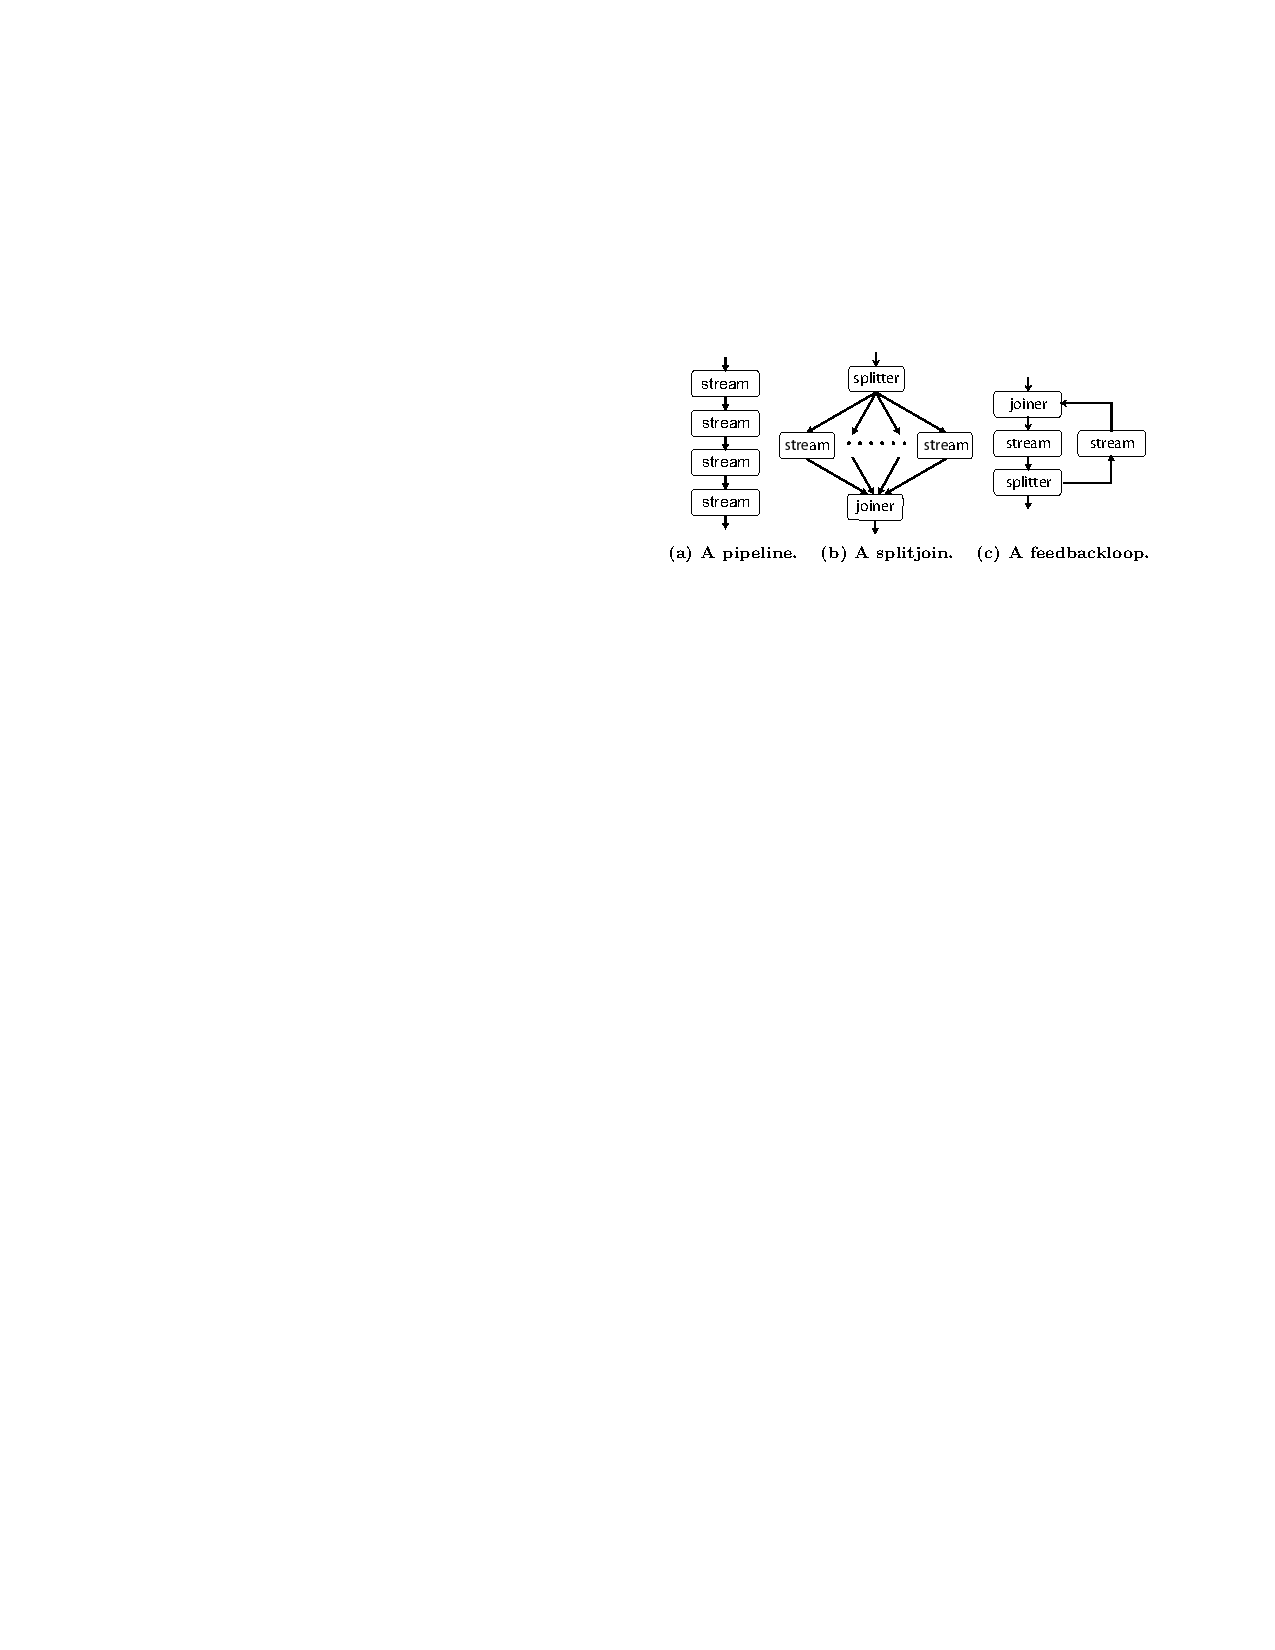
\includegraphics[width=3.3in]{stream-structures.pdf}
%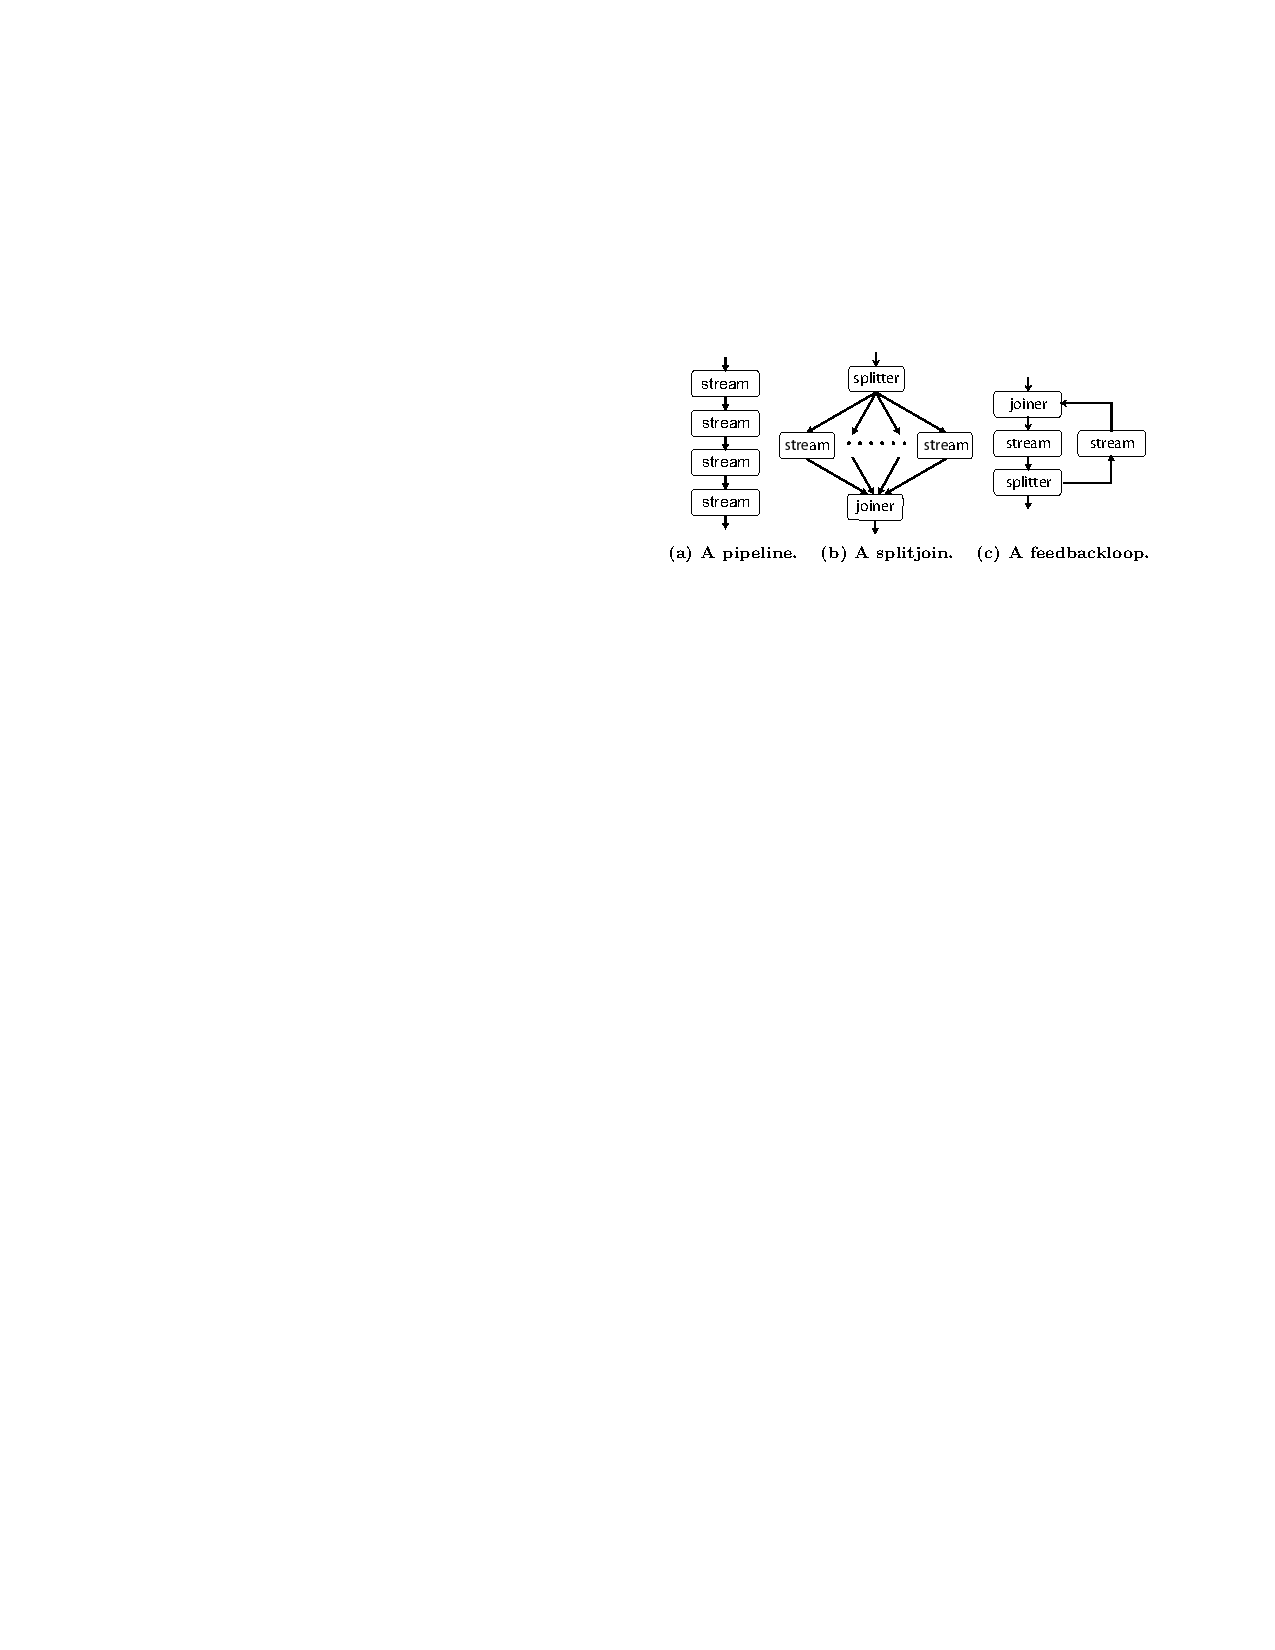
\psfig{file=stream-structures,width=\columnwidth}
\caption{Hierarchical stream structures supported by StreamIt.\protect\label{fig:structures}}
\end{figure}

The StreamIt compiler coarsens the granularity of a stream graph by
applying the {\it fusion} transformation which merges adjacent filters
into a single (large) filter (embedding the schedules of execution in
the merged filter)~\cite{streamit-asplos}.  The {\it fission}
transformation is employed to add data parallelism to a stream graph.
In fission, a single filter without state is duplicated a certain
number of ways and placed in a splitjion construct.  Input items to
the original filter are distributed among the duplicates, termed {\it
  fission products}.  In \S\ref{sec:fission}, we describe how to
extend the fundamental fission transformation to parallelize induction
variable state.

  \begin{figure*}[th]
\vspace{-12pt}
\begin{minipage}{3.2in}
\begin{center}
\begin{minipage}{0.46in}
\centering
\psfig{figure=pipeline.eps,width=0.46in} \\
\end{minipage} 
~
\begin{minipage}{1.3in}
\centering
\psfig{figure=splitjoin.eps,width=1.3in} \\
\end{minipage}
~
\begin{minipage}{1.02in}
\centering
\psfig{figure=feedback.eps,width=1.02in} \\
\end{minipage} 
\\ ~ \\ {\protect\small (a) A pipeline. ~~(b) A splitjoin. ~~(c) A feedbackloop.}
\caption{Stream structures supported by StreamIt.
\protect\label{fig:structures}}
\end{center}
\end{minipage}
~~~~~
\begin{minipage}{3in}
\centering
\vspace{15pt}
\psfig{figure=raw-diagram.eps,width=3in}
\caption{Block diagram of the Raw architecture.
\protect\label{fig:raw-diagram}}
\end{minipage}
\vspace{-12pt}
\end{figure*}

\section{The Raw Architecture}
\label{sec:raw}

The Raw Microprocessor \cite{raw10,raw} addresses the wire delay
problem \cite{raw13} by providing direct instruction set architecture
(ISA) analogs to three underlying physical resources of the processor:
gates, wires and pins. Because ISA primitives exist for these
resources, a compiler such as StreamIt has direct control over both
the computation and the communication of values between the functional
units of the microprocessor, as well as across the pins of the
processor.

The architecture exposes the gate resources as a scalable 2-D array of
identical, programmable tiles, that are connected to their immediate
neighbors by four on-chip networks.  Values routed through the
networks off of the side of the array appear on the pins, and values
placed on the pins by external devices (wide-word A/Ds, DRAMS, etc.)
appear on the networks.  Each of the tiles contains a compute
processor, some memory and two types of routers--one static, one
dynamic--that control the flow of data over the networks as well as
into the compute processor (see Figure \ref{fig:raw-diagram}).  The
compute processor interfaces to the network through a bypassed,
register-mapped interface \cite{raw10} that allows instructions to use
the networks and the register files interchangeably.

Each tile's static router has a virtualized instruction memory to
control the crossbars of the two static networks. Collectively, the
static routers can reconfigure the communication pattern across these
networks every cycle.  The input and output possibilities for each
crossbar are: North, East, South, West, Processor, to the other
crossbar, and into the static router. The FIFOs are typically four or
eight elements large.  To route a word from one tile to another, the
compiler inserts a route instruction on every intermediate static
router.  Because the routers are pipelined and compile-time scheduled,
they can deliver a value from the ALU of one tile to the ALU of a
neighboring tile in 3 cycles, or more generally, 2+N cycles for an
inter-tile distance of N hops.

Because we generate regular bulk DRAM transfers, we did not want
accesses to off-chip memory to become the bottleneck of the hardware
configuration.  So, we use a simulation of a CL2 PC 3500 DDR DRAM,
which provides enough bandwidth to saturate both directions of a Raw
port \cite{raw_isca}.  In our configuration, we use 16 such DRAMs,
attached to each of the 16 logical ports of the chip.  Also, we
implemented a streaming memory controller in the chipset that supports
a number of simple streaming memory requests.  The chipset receives
request messages over the general dynamic network for bulk transfers
to and from the DRAMs.  The transfers themselves can use either the
static network or the general dynamic network (the desired network is
encoded in the request).  Simple interleaving and striding is
supported by the chipset, but is unused by the Spacetime Compiler,
since all DRAM accesses are to or from a contiguous chuck of memory
with unit stride. The chipsets also have a simple demultiplexing
mechanism that allows multiple devices (such as external input and
output streams) to share a single port.

The results of this paper were generated using btl, a cycle-accurate
simulator that models arrays of Raw tiles identical to those in the
.15 micron 16-tile Raw prototype ASIC chip.  With a target clock rate
of 450 MHz, the tile employs as compute processor an 8-stage, single
issue, in-order MIPS-style pipeline that has a 32 KB data cache, 32 KB
of instruction memory, and 64 KB of static router memory.

(FileReaders and writers should be talked about as connected to the
bypass port of the dram chipset).
  \section{Compiling StreamIt to Raw}
\label{sec:phases}

\begin{table}[t]
\begin{center}
\scriptsize
\begin{tabular}{|l|l|} \hline
{\bf Phase} & {\bf Function} \\
\hline \hline
KOPI Front-end & Parses syntax into a Java-like abstract syntax tree. \\
\hline
SIR Conversion & Converts the AST to the StreamIt IR (SIR). \\
\hline
Graph Expansion & Expands all parameterized structures in the stream graph. \\
\hline
Scheduling & Calculates initialization and steady-state execution orderings for filter firings. \\
\hline
Partitioning & Performs fission and fusion transformations for load balancing. \\
\hline
Layout & Determines minimum-cost placement of filters on grid of Raw tiles. \\
\hline
Communication Scheduling & Orchestrates fine-grained communication between tiles via simulation of the stream graph. \\
\hline
Code generation & Generates code for the tile and switch processors. \\
\hline
\end{tabular}
\vspace{-6pt}
\caption{\protect\small Phases of the StreamIt compiler.
\label{tab:phases}}
\vspace{-12pt}
\end{center}
\end{table}

The phases of the StreamIt compiler are described in
Table~\ref{tab:phases}.  The front end is built on top of KOPI, an
open-source compiler infrastructure for Java~\cite{kopi}.  We
translate the KOPI syntax tree into the StreamIt IR (SIR) that
encapsulates the hierarchical stream graph.  Since the structure of
the graph might be parameterized, we propagate constants and expand
each stream construct to a static structure of known extent.  At this
point, we can calculate an execution schedule for the nodes of the
stream graph.

The automatic scheduling of the stream graph is one of the primary
benefits that StreamIt offers, and the subtleties of scheduling and
buffer management are evident throughout all of the following phases
of the compiler.  The scheduling is complicated by StreamIt's support
for the {\tt peek} operation, which implies that some programs require
a separate schedule for initialization and for the steady state.  The
steady state schedule must be periodic--that is, its execution must
preserve the number of live items on each channel in the graph (since
otherwise a buffer would grow without bound.)  A separate
initialization schedule is needed if there is a filter with $peek >
pop$, by the following reasoning.  If the initialization schedule were
also periodic, then after each firing it would return the graph to its
initial configuration, in which there were zero live items on each
channel.  But a filter with $peek > pop$ leaves $peek-pop$ (a positive
number) of items on its input channel after {\it every} firing, and
thus could not be part of this periodic schedule.  Therefore, the
initialization schedule is separate, and non-periodic.

In the StreamIt compiler, the initialization schedule is constructed
via symbolic execution of the stream graph, until each filter has at
least $peek-pop$ items on its input channel.  For the steady state
schedule, there are many tradeoffs between code size, buffer size, and
latency, and we are developing techniques to optimize different
metrics \cite{streamittech2}.  In this paper, we use a simple
hierarchical scheduler that constructs a Single Appearance Schedule
(SAS) \cite{leesdf} for each filter.  An SAS is one where each node
appears exactly once in the loop nest denoting the schedule.  We
construct one such loop nest for each hierarchical stream construct,
such that each component is executed a set number of times for every
execution of its parent.  In later sections, we refer to the
``multiplicity'' of a filter as the number of times that it executes
in one steady state execution of the entire stream graph.

Following the scheduler, the compiler has stages that are specific for
communication-exposed architectures: partitioning, layout, and
communication scheduling.  The next three sections of the paper are
devoted to these phases.




  \begin{figure}
  \vspace{-18pt}
  \begin{center} \psfig{figure=beam-blood-key.eps,width=3.25in} \\
    \subfigure[\vspace{-12pt}
    Original.\label{fig:fm-blood1}]{\psfig{figure=radio-blood-orig.eps,width=3in}\vspace{-12pt}}
    \hspace{0.3in} \subfigure[\vspace{-12pt}
    Load-balanced.\label{fig:fm-blood2}]{\psfig{figure=radio-blood-opt.eps,width=3in}\vspace{-12pt}}
    \vspace{-12pt} \caption{Execution traces for the (a)
    original and (b) load-balanced partitionings of the FM Radio.  The
    $x$ axis denotes time, and the $y$ axis denotes the processor.
    The dark bands indicate periods where processors are blocked
    waiting to receive an input or send an output.  Light regions
    indicate periods of useful work.  The thin stripes in the light
    regions represent pipeline stalls.  \protect\label{fig:fm-blood}}
    \vspace{-6pt}
\end{center}
\vspace{-18pt}
\begin{minipage}{3.2in}
\centering
\psfig{figure=radio-graph-orig.eps,width=3in}
\parbox{2.75in}{
\caption{\protect\small Stream graph of the original FM Radio, in
which the Filters are at a granularity that is natural for the
algorithm. \protect\label{fig:fm-orig}}}
\end{minipage}
\hspace{0.1in}
\begin{minipage}{3.2in}
\centering
\vspace{0.5in}
\psfig{figure=radio-graph-opt.eps,width=3in}
\parbox{2.75in}{
\caption{\protect\small Stream graph of the load-balanced FM Radio.
Since the first LowPassFilter was the most demanding node, it was
duplicated across a 2-way SplitJoin.  Then, to conserve tiles, the
Subtract node was hoisted across a downstream Joiner, and the
Subtract, Add, and Printer nodes were fused.\protect\label{fig:fm-opt}}}
\end{minipage}
\end{figure}

\section{Partitioning}
\label{sec:partition}

StreamIt provides the Filter construct as the basic abstract unit of
autonomous stream computation.  The programmer should decide the
boundaries of each Filter according to what is most natural for the
algorithm under consideration.  While one could envision each Filter
running on a separate machine in a parallel system, StreamIt hides the
granularity of the target machine from the programmer.  Thus, it is
the responsibility of the compiler to adapt the granularity of the
stream graph for efficient execution on a particular architecture.

We use the word {\it partitioning} to refer to the process of dividing
a stream program into a set of balanced computation units.  Given a
number $N$, which represents the maximum number of computation units
that can be supported, the partitioning stage transforms a stream
graph into a set of no more than $N$ filters, each of which performs
approximately the same amount of work during the execution of the
program.  Following this stage, each filter can be run on a separate
processor to obtain a load-balanced executable.

Load balancing is particularly important in the streaming domain,
since the throughput of a stream graph is equal to the {\it minimum}
throughput of each of its stages.  This is in contrast to scientific
programs, which often contain a number of stages which process a given
data set; the running time is the {\it sum} of the running times of
the phases, such that a high-performance, parallel phase can partially
compensate for an inefficient phase.  In mathematical terms, Amdahl's
Law captures the maximum realizable speedup for scientific
applications.  However, for streaming programs, the maximum
improvement in throughput is given by the following expression:
\begin{align*}
\mbox{\it Maximum speedup}(w, c) = \frac{\sum_{i=1}^N{w_i \cdot c_i}}{MAX_i(w_i \cdot c_i)}
\end{align*}
where $w_1 \dots w_m$ denote the amount of work in each of the $N$
partitions of a program, and $c_i$ denotes the multiplicity of work
segment $i$ in the steady-state schedule.  Thus, if we double the load
of the heaviest node ({\it i.e.}, the node with the maximum $w_i \cdot
c_i$), then the performance could suffer by as much as a factor of
two.  The impact of load balancing on performance places particular
value on the partitioning phase of a stream compiler.
% This can be posed in
% mathematical terms by appealing to Amdahl's Law, which expresses the
% maximum speedup that can be achieved on $N$ processors when there are
% $S_1 \dots S_x$ units of sequential work and $P_1 \dots P_y$ units of
% parallel work:
% \begin{align*}
% \mbox{\it Maximum speedup}(S, P, N) = \frac{\sum_{i=1}^x{S_i}+\sum_{i=1}^y{P_i}}{\sum_{i=1}^x{S_i}+\frac{\sum_{i=1}^y{P_i}}{N}}
% \end{align*}
% However, in a stream program, the measure of performance is throughput
% rather than running time.  Using $w_1 \dots w_m$ to denote the amount
% of work in each of the $m$ partitions of a program, and denoting the
% multiplicity of work segment $i$ in the steady-state schedule by
% $c_i$, we have that:

\subsection{Overview}

Our partitioner employs a set of fusion, fission, and reordering
transformations to incrementally adjust the stream graph to the
desired granularity.  To achieve load balancing, the compiler
estimates the number of instructions that are executed by each filter
in one steady-state cycle of the entire program; then, computationally
intensive filters can be split, and less demanding filters can be
fused.  Currently, the decision of which transformations to apply is
done by hand, but the transformations themselves are fully automated.

We use the FM Radio application to illustrate the partitioning
process.  The original partitioning of the radio
(Figure~\ref{fig:fm-orig}) is highly unbalanced, as the first
LowPassFilter node constitutes a large fraction of the work in the
stream graph.  Figure~\ref{fig:fm-blood1} provides an execution trace
of the original partitioning and demonstrates that this filter is the
bottleneck for the computation.  The StreamIt compiler performs
horizontal fission, filter hoisting, and vertical fusion
transformations to obtain the improved stream graph given in
Figure~\ref{fig:fm-opt}.  As illustrated by the execution trace in
Figure~\ref{fig:fm-blood2}, the load-balanced graph achieves more than
twice as much processor utilization as the original, since the
computationally intensive nodes have been split and the lighter nodes
have been combined. In the following sections, we describe these
transformations in more detail.

\begin{figure}
\centering
\psfig{figure=fuse-pipeline.eps,width=6.5in}
\vspace{-6pt}
\caption{\protect\small Fusion of a Pipeline into a two-stage filter.
In this example, the UpSampler pushes $K$ items on every step, while the
MovingAverage filter peeks at $N$ items but only pops 1.  To accommodate
this peeking behavior, the fused filter maintains a {\tt peek\_buffer}
for the items that reside on the channel between the two filters.  In
the initial work function, which is called only on the first
invocation, the {\tt peek\_buffer} is filled with initial values from
the UpSampler.  The steady work function implements a steady-state
schedule in which $\mt{LCM}(N, K)$ items are transferred between the two
original filters--these items are communicated through a local,
temporary {\tt buffer}.  Before and after the execution of the
MovingAverage code, the contents of the {\tt peek\_buffer} are
transferred in and out of the temporary {\tt buffer}.  If the {\tt
peek\_buffer} is small, this copying can be eliminated with loop
unrolling and copy propagation.  Note that the {\tt peek\_buffer} is
for storing items that are persistent from one firing to the next,
while the local {\tt buffer} is just for communicating values during a
single firing. \label{fig:fuse-pipe}}
\vspace{-6pt}
\end{figure}

\subsection{Fusion Transformations}

Filter fusion is a transformation whereby several adjacent filters are
combined into one.  Fusion can be applied to decrease the granularity
of a stream graph so that an application will fit on a given target,
or to improve load balancing by merging small filters so that there is
space for larger filters to be split.  Analogous to loop fusion in the
scientific domain, filter fusion can enable other optimizations by
merging the control flow graphs of adjacent nodes, thereby shortening
the live ranges of variables and allowing independent instructions to
be reordered.

\subsubsection{Vertical Fusion}

Vertical fusion describes the combination of sequential, pipelined
filters into a single unit.  We have developed a vertical fusion
algorithm for StreamIt filters that we describe below.  For the more
limited domain of filters that do not contain peek statements,
Proebsting and Watterson \cite{pro96} present a filter fusion
algorithm that interleaves the control flow graphs of adjacent nodes.
However, they assume that nodes communicate via synchronous {\tt get}
and {\tt put} operations, such that StreamIt's asynchronous peek
operations and implicit buffer management fall outside the scope of
their model.

Our algorithm relies on the static I/O rates of each filter to
calculate a legal execution ordering for the filters being fused.
Then, the fused filter simulates the execution of this schedule,
inlining the code from each of the original filters and using local
variables for buffering.  In our current implementation, the scheduler
computes only the multiplicity of each component filter in relation to
the fused filter; then, the fused code is a sequence of loops that
each execute a component filter for the appropriate multiplicity,
buffering its results in a local array.  If the multiplicity is small,
then the loop can be unrolled and all array references can be replaced
with scalar variables to facilitate optimization.

A subtlety of our algorithm is that the fused filter differs from the
originals in that it has two distinct execution phases: one for
initialization, and one for steady-state execution (see
Figure~\ref{fig:fuse-pipe}).  If any of the component filters peek at
elements that they do not consume, then a separate initialization
schedule is required to fill all the ``peek buffers'' in the pipeline
(see Section~\ref{sec:phases}).  During this initialization, the
pipeline as a whole will consume some input, but will not produce any
output.  Then, during the steady state schedule, the sizes of the
buffers are preserved, and the pipeline both produces and consumes
items.  Thus, when there is peeking in the stream, there will be
different I/O rates for the initialization and steady-state phases,
and the fused filter will be a {\it two stage filter}: it executes one
work function on its first invocation, and a separate work function on
all subsequent invocations.  Though these work functions may have
different I/O rates, each rate is constant and known at compile time.

\subsubsection{Horizontal Fusion}

We refer to the combination of the parallel streams in a SplitJoin
construct as ``horizontal fusion''.  Our horizontal fusion algorithm
inputs a SplitJoin where each component is a single filter, and
outputs a Pipeline of three filters: one to emulate the Splitter, one
to simulate the execution of the parallel filters, and one to emulate
the Joiner.  The Splitters and Joiners need to be emulated in case
they are RoundRobin's that perform some reordering of the data items
with respect to the component streams.  Generally speaking, the fusion
of the parallel components is similar to that of vertical fusion--a
sequential steady-state schedule is calculated, and the component work
functions are inlined and executed within loops.  However, horizontal
fusion requires no buffering of internal items, as the parallel
streams do not communicate with each other.

\begin{figure}
\centering
\psfig{figure=fuse-splitjoin.eps,width=4.93in}
\caption{\protect\small Fusion of a Duplicate SplitJoin construct.  To
fuse a SplitJoin with a Duplicate Splitter, the code of the component
filters is inlined into a single filter with repetition according to
the steady-state schedule.  However, there are some modifications: all
{\tt pop} statements are converted to {\tt peek} statements, and the
{\tt pop}'s are performed at the end of the fused work function.  This
allows all the filters to see the data items before they are consumed.
Finally, the RoundRobin Joiner is simulated by a ReorderRoundRobin
filter that re-arranges the output of the fused filter according to
the weights of the Joiner.  \protect\label{fig:fuse-splitjoin1}}
\vspace{18pt}
\psfig{figure=fuse-splitjoin2.eps,width=4.93in}
\caption{\protect\small Fusion of a RoundRobin SplitJoin construct.
The fusion transformation for SplitJoins containing RoundRobin
Splitters is similar to those containing Duplicate Splitters.  One
filter simulates the execution of a steady-state cycle in the
SplitJoin by inlining the code from each filter.  This filter is
surrounded by ReorderRoundRobin filters that recreate the reordering of
the RoundRobin nodes.  In the above example, the difference the
Splitter's weights, the Filter's I/O rates, and the Joiner's weights
adds complexity to the reordering.  Though this transformation is
fully automated in the StreamIt compiler, a general formulation is
beyond the scope of this paper.  \protect\label{fig:fuse-splitjoin2}}
\end{figure}

The details of our horizontal fusion transformation depend on the type
of the Splitter in the construct of interest.  There are two cases:
\begin{enumerate}
\item For {\bf Duplicate} Splitters, the {\tt pop} expressions from
component filters need to be converted to {\tt peek} expressions so
that items are not consumed before subsequent filters can read them
(see Figure~\ref{fig:fuse-splitjoin1}).  Then, at the end of the fused
work function, the items consumed by an iteration of the SplitJoin are
popped from the input channel.  Also, the Splitter itself performs no
reordering of the data, so it translates into an Identity filter that
can be removed from the stream graph.  This fusion transformation is
valid even if the component Filters peek at items which they do not
consume.

\item For {\bf RoundRobin} Splitters, the {\tt pop} expressions in
component filters are left unchanged, and the RoundRobin Splitter is
emulated in order to reorder the data items according to the weights
of the Splitter and the consumption rates of the component streams
(see Figure~\ref{fig:fuse-splitjoin2}).  However, this transformation
is invalid if any of the component Filters peeks at items which it
does not consume, since the interleaving of items on the input stream
of the fused filter prevents each component from having a continuous
view of the items that are intended for it.  Thus, we only apply this
transformations when all component Filters have $peek = pop$.
\end{enumerate}

A more mathematical description of our horizontal fusion
transformation is given in \cite{streamittech2}.

\begin{figure}
\centering
\psfig{figure=duplicate-fission-2.eps,width=4.60in}
\caption{\protect\small Fission of a filter that does not peek.  For
Filters such as a VectorMultiply that consumes every item they look
at, horizontal fission consists of embedding copies of the filter in a
$K$-way RoundRobin SplitJoin.  The weights of the Splitter and Joiner
are set to match the $pop$ and $push$ rates of the filter,
respectively.  \protect\label{fig:fission-nopeek}}
\vspace{18pt}
\psfig{figure=duplicate-fission.eps,width=3.94in}
\caption{\protect\small Fission of a filter that peeks.  Since the
MovingAverage filter reads items that it does not consume, the
duplicated versions of the filter need to access overlapping portions
of the input stream.  For this reason, horizontal fission creates a
Duplicate SplitJoin in which each component filter has additional code
to filter out items that are irrelevant to a given path.  This
decimation occurs in two places: once in the initial work function, to
disregard items considered by previous filters on the first iteration
of the SplitJoin, and once at the end of the steady work function, to
account for items consumed by other components.
\protect\label{fig:fission-peek}}
\end{figure}

\subsection{Fission Transformations}

Filter fission is the analog of parallelization in the streaming
domain.  It can be applied to increase the granularity of a stream
graph to utilize unused processor resources, or to break up a
computationally intensive node for improved load balancing.

\subsubsection{Vertical Fission}

Some filters can be split into a pipeline, with each stage performing
some part of the {\tt work} function.  In addition to the original
input data, these pipelined stages might need to communicate
intermediate results from within {\tt work}, as well as fields within
the filter.  This scheme could apply to filters with state if all
modifications to the state appear at the top of the pipeline (they
could be sent over the data channels), or if changes are infrequent
(they could be sent via StreamIt's messaging system.)  Also, some
state can be identified as induction variables, in which case their
values can be reconstructed from the {\tt work} function instead of
stored as fields.  We have yet to automate vertical filter fission in
the StreamIt compiler.

\subsubsection{Horizontal Fission}

We refer to ``horizontal fission'' as the process of distributing a
single filter across the parallel components of a SplitJoin.  We have
implemented this transformation for ``stateless'' filters--that is,
filters that contain no fields that are written on one invocation of
{\tt work} and read on later invocations.  Let us consider such a
filter $F$ with I/O rates of $peek$, $pop$, and $push$, that is being
parallelized into an $K$-way SplitJoin.  There are two cases to
consider:
\begin{enumerate}
\item If {\bf $peek = pop$}, then $F$ can simply be duplicated $K$
ways in the SplitJoin (see Figure~\ref{fig:fission-nopeek}).  The
Splitter is a RoundRobin that routes $pop$ elements to each copy of
$F$, and the Joiner is a RoundRobin that reads $push$ elements from
each component.  Since $F$ does not peek at any items which it does
not consume, its code does not need to be modified in the component
streams--we are just distributing the invocations of $F$.

\item If {\bf $peek > pop$}, then our transformation produces a
SplitJoin that has a set of two-stage filters as its components (see
Figure~\ref{fig:fission-peek}).  In this case, the Splitter is a
Duplicate, since the component filters need to examine overlapping
parts of the input stream.  The $i$'th component has a steady-state
work function that begins with the work function of $F$, but appends a
series of $(K-1)*pop$ pop statements in order to account for the data
that is consumed by the other components.  Also, the $i$'th filter has
an initialization work function that pops $(i-1)*pop$ items from the
input stream, to account for the consumption of previous filters on
the first iteration of the SplitJoin.  As before, the Joiner is a
RoundRobin that has a weight of $push$ for each stream.
\end{enumerate}

\begin{figure}
\centering
\psfig{figure=filter-hoisting.eps,width=4.81in}
\caption{\protect\small Filter hoisting.  This transformation allows a
stateless Filter to be moved across a Joiner node if its $push$ value
evenly divides the weights of the Joiner.  This proved to be useful in
load balancing the FMRadio application.
\protect\label{fig:filter-hoisting}}
\vspace{12pt}
\psfig{figure=splitjoin-split.eps,width=5.13in}
\caption{\protect\small Breaking a SplitJoin into hierarchical units.
Though our horizontal fusion algorithms work on the granularity of an
entire SplitJoin, it is straightforward to transform a large SplitJoin
into a number of smaller pieces, as shown here.  Following this
transformation, the fusion algorithms can be applied to obtain an
intermediate level of granularity.  This technique was employed to
help load-balance the BeamFormer (see Section~\ref{sec:results}).
\protect\label{fig:splitjoin-split}}
\vspace{12pt}
\psfig{figure=sync-removal.eps,width=4.02in}
\caption{\protect\small Synchronization removal.  If a Splitter is
bordering a Joiner with identical weights, the nodes can be removed
and the component streams can be connected.  This is especially useful
in the context of libraries--many distinct components can employ
SplitJoins for processing interleaved data streams, and the modules
can be composed without having to synchronize all the streams at each
boundary.  \protect\label{fig:sync-removal}}
\vspace{-6pt}
\end{figure}

\subsection{Reordering Transformations}
There are a multitude of ways to reorder the elements of a stream
graph so as to facilitate fission and fusion transformations.  For
instance, identical stateless filters can be pushed through a Splitter
or Joiner node if the weights are adjusted accordingly
(Figure~\ref{fig:filter-hoisting}); a SplitJoin construct can be
divided into a hierarchical set of SplitJoins to enable a finer
granularity of fusion (Figure~\ref{fig:splitjoin-split}); and
neighboring Splitters and Joiners with matching weights can be
eliminated (Figure~\ref{fig:sync-removal}).  Many of these
transformations were useful in load balancing our test applications.

\subsection{Summary}

We have described fission and fusion transformations for a large
domain of stream constructs.  Our vertical fusion transformation
applies to any sequence of filters, with or without peeking; our
horizontal fusion transformation supports peeking if the Splitter is a
Duplicate, but not if the Splitter is a RoundRobin.  Our horizontal
fission algorithm duplicates any stateless filter into a SplitJoin
construct of arbitrary width.

The one domain that we have left unexplored is the fusion and fission
of two-stage filters.  If a two-stage filter (with a non-empty initial
work function) results from one transformation, then no subsequent
transformations can be safely performed on them.  We are currently
extending our transformations to support two-stage filters.




  \section{Slice Layout}
Simulated annealing

3-D bin packing problem 
	how it differs
prior solutions
	GA
	SA
	hard to say what is good
What we use
	SA
	adaptive annealing schedule 
	
3d visualization????
  \begin{figure}
\centering
\psfig{figure=joiner-buffer-dead.eps,width=4.59in}
\parbox{6in}{\caption{\protect\small Example of deadlock in a
SplitJoin.  As the Joiner is reading items from the stream on the
left, items accumulate in the channels on the right.  On Raw, senders
will block once a channel has four items in it.  Thus, once 10 items
have passed through the Joiner, the system is deadlocked, as the
Joiner is trying to read from the left, but the stream on the right is
blocked.  The Identity filter is blocking on the send of item \#10,
and the Splitter is blocking on the send of item \#20.  If the weights
on the Joiner were (10, 10), the system would be deadlock-free.
\protect\label{fig:joiner-dead}}}

\vspace{48pt}

\psfig{figure=joiner-buffer-live.eps,width=3.97in}
\caption{\protect\small Fixing the deadlock with a buffering Joiner.
The BufferingRoundRobin is an internal StreamIt construct (it is not
part of the language) which reads items from its input channels in the
order in which they arrive, rather than in the order specified by its
weights.  The order of arrival is determined by a simulation of the
stream graph's execution; thus, the system is guaranteed to be
deadlock-free, as the order given by the simulation is feasible for
execution on Raw.  To preserve the semantics of the Joiner, the items
are written to the output channel from the internal buffers in the
order specified by the Joiner's weights.  The ordered items are sent
to the output as soon as they become available.
\protect\label{fig:joiner-live}}
\end{figure}

\section{Communication Scheduler}
\label{sec:communic}

With the nodes of the stream graph assigned to computation nodes of
the target, the next phase of the compiler must map the communication
explicit in the stream graph to the interconnect of the target.  This
is the task of the communication scheduler.  The communication
scheduler maps the infinite FIFO abstraction of the stream channels to
the limited resources of the target.  The communication scheduler must
avoid deadlock and starvation while trying to utilize the parallelism
explicit in the stream graph.

The exact implementation of the communication scheduler is tied to the
communication model of the target.  The simplest mapping would occur
for targets implementing an end-to-end, infinite FIFO abstraction, in
which the scheduler needs only to determine the sender and receiver of
each data item.  This information is easily calculated from the
weights of the Splitters and Joiners.  As the communication model
becomes more constrained, the communication scheduler becomes more
complex, requiring analysis of the stream graph. For targets
implementing a finite, blocking nearest-neighbor communication model,
the exact ordering of tile execution must be specified.

Due to the static nature of StreamIt, the compiler can statically
orchestrate the communication resources.  As described in
Section~\ref{sec:phases}, we create an initialization schedule and a
steady-state schedule that fully describe the execution of the stream
graph.  The schedules can give us an order for execution of the graph
if necessary.  We can generate ordering to minimize buffer length,
maximize parallelism, or minimize latency.

%Thus, we can create a communication scheduler of arbitrary
%detail.  If the architecture must statically orchestrate all aspects
%of communication, the StreamIt language provides this facility.

Deadlock must be carefully avoided in the communication
scheduler. Each architecture requires a different deadlock avoidance
mechanism and we will not go into a detailed explanation of deadlock
here.  In general, deadlock occurs when there is a circular dependence
on resources.  A circular dependence can surface in the stream graph
or in the routing pattern of the layout.  If the architecture does not
provide sufficient buffering, the scheduler must serialize all
potentially deadlocking dependencies.

%Two StreamIt language constructs that can lead to deadlock are
%FeedbackLoops and Joiners. Figure ?? describes the potential for
%deadlock in a FeedbackLoop.  One potential solution is to forbid
%filters of the FeedbackLoop to interleave sends and receives.  This
%has the effect of serializing the FeedbackLoop. In figure ?? we
%descibe the potential for deadlock introduced by Joiner nodes.  A
%solution to this problem is described below.

\subsection{Communication Scheduler for Raw}
\label{sec:rawcommunic}

The communication scheduling phase of the StreamIt compiler maps
StreamIt's channel abstraction to Raw's static network.  As mentioned
in Section \ref{sec:raw}, Raw's static network provides optimized,
nearest neighbor communication.  Tiles communicate using buffered,
blocking sends and receives.  It is the compiler's responsibility to
statically orchestrate the explicit communication of the stream graph
while preventing deadlock.

To statically orchestrate the communication of the stream graph, the
communication scheduler simulates the firing of nodes in the stream
graph, recording the communication as it simulates.  The simulation
does not model the code inside each Filter; instead it assumes that
each Filter fires instantaneously.  This relaxation is possible
because of the flow control of the static network--since sends block
when a channel is full and receives block when a channel is empty, the
compiler needs only to determine the ordering of the sends and
receives rather than arranging for a precise rendezvous between sender
and receiver.

% We simulate the graph for both an initialization schedule and a steady
% state schedule (see Section \ref{sec:phases}).  A ``push schedule'' is
% used for both phases.  We define a push schedule as one that always
% fires the node that is the furthest downstream (among those that have
% enough inputs to fire).  
% 
% A push schedule allows the implementation to
% disregard the FIFO buffers that connect each neighboring node in the
% stream graph.  This is because data items will not be accumulating at
% the source, dest, or intermediate nodes.  Each destination will
% consume the data item as it is produced (modulo the latency of
% routing).

Special care is required in the communication scheduler to avoid
deadlock in SplitJoin constructs.  Figure~\ref{fig:joiner-dead}
illustrates a case where the naive implementation of a SplitJoin would
cause deadlock in Raw's static network.  The fundamental problem is
that some SplitJoins require a buffer of values at the Joiner
node--that is, the Joiner outputs values in a different order than it
receives them.  This can cause deadlock on Raw because the buffers
between channels can hold only four elements; once a channel is full,
the sender will block when it tries to write to the channel.  If this
blocking propagates the whole way from the Joiner to the Splitter,
then the entire SplitJoin is blocked and can make no progress.

To avoid this problem, the communication scheduler implements internal
buffers in the Joiner node instead of exposing the buffers on the Raw
network (see Figure~\ref{fig:joiner-live}).  As the execution of the
stream graph is simulated, the scheduler records the order in which
items arrive at the Joiner, and the Joiner is programmed to fill its
internal buffers accordingly.  At the same time, the Joiner outputs
items according to the ordering given by the weights of the
RoundRobin.  That is, the sending code is interleaved with the
receiving code in the Joiner; no additional items are input if a
buffered item can be written to the output stream.  To facilitate code
generation (Section \ref{sec:codegen}), the maximum buffer size of
each internal buffer is recorded.

Our current implementation of the communication scheduler is overly
cautious in its deadlock avoidance.  All FeedbackLoops are serialized
by the communication scheduler to prevent deadlock.  More precisely,
the loop and body streams of each FeedbackLoop cannot execute in
parallel.  Crossed routes in the layout of the graph are serialized as
well, forcing each path to wait its turn at the contention point.
	
  \section{Code Generation}
\label{sec:codegen}
In this section we consider low-level code generation for the Raw
microprocessor. Each Raw tile is an amalgam of the filters that
execute on it. To generate the execution code for the entire
application, we traverse the schedule for each phase of computation:
first the peek initialization stage, then prologue stage, and finally
the steady-state.  As we traverse each schedule, we generate the
computation and communication code as we visit each slice.  For the
initialization and prologue stages, we do a traversal of the slice
graph that respects the data-dependencies stipulated by the stream
graph. For the steady-state we traverse the schedule as calculated by
the slice scheduling algorithm of Section \ref{sec:scheduling}.

When we visit a slice, we first generate the DRAM requests and
communication code load its inputs from and store its outputs to its
mapped off-chip DRAM.  Next, we generate computation and communication
code for each filter of the slice.  

\subsection{Slice Data Reordering}
Before a steady-state execution can commence, each slice's single
input stream must be assembled in the order stipulated by the
round-robin weights on its incoming channels. To achieve this, the
various input streams of the slices are collected into the memory
module attached to the tile to which the first filter of the slice is
mapped. Streaming DRAM requests are generated to read each input
channel and to write the final, reassembled input.  Code is generated
for the static routers, as they perform the ordering of the final
input stream as stipulated by each joiner.  Splitting is done in much
the same way.  The compute processor of Raw are idle during
data-reorganization stage.

Remember from Section \ref{sec:softpipe} that the source and
destination buffers of this stage are the rotating buffers that
facilitate the software pipeline.  The number of individual memory
blocks that compose the rotating buffer is determined by the
multiplicity difference between the source slice and destination slice
in the prologue schedule.  Each time an off-chip memory request is
issued, the buffer will rotate, with two rotation structures for each
buffer that rotate separately, one for reading and one for writing.

\subsection{Filter Code Generation}
We generate computation and communication code for the individual
filters of the slice in much the same way as \cite{streamit-asplos}.  
%When we visit a slice in the schedule for each execution phase, we
%iterate over the filters that compose the slice, generating 
%communication and computation code necessary to execute the slice.
%The scheduling phase (Section \ref{sec:scheduling}) produces a mapping
%of filters to tiles.

%\subsubsection{Compute Processor}
%%For linear slices, we generate parameterized, template assembly code
%%for both computation and communication as described in Section
%%\ref{sec:linear}.  
%As we iterate over the filters of the slice, we append the code
%necessary to execute the current filter to the existing code for the
%tile to which the filter is mapped.  We also make sure to execute the
%{\tt init} function of each filter before we start the peek
%initialization stage. Consequently, each compute processor begins by
%calling the {\tt init} function of all the filters mapped to it.
%Next, the compute processor executes the {\tt work} function of each
%filter assigned to it in sequence.  The sequence is determined by the
%traversal of the schedule of each execution phase; first the
%peek initialization stage, then the prologue stage, and finally the
%steady-state.  Each work function execution is placed in a loop that
%executes the number of times the filter fires in the current stage.

%For Raw's compute processor, we generate a mixture of C code
%and assembly instructions that is compiled using Raw's GCC 3.3
%port. The translation of the {\tt init} function, {\tt work}
%functions, and any helper function is, for the large part,
%straightforward.  Most StreamIt expression have direct analogs in C
%except for the channel expressions {\tt push()}, {\tt peek(index)} and
%{\tt pop()}.

%One major benefit of StreamIt over other streaming languages is that
%the StreamIt compiler is responsible for buffer management.  The
%programmer is free to call {\tt pop()} or {\tt peek(index)} without
%having to worry about the structure of the buffer or updating the
%buffer's index variable after each execution of the work function.
%Currently, we classify filters as one of three types with respect to
%buffer management:
%\begin{enumerate}
%\item If a filter $(i)$ does not contain any {\tt peek} statements, $(ii)$
%does not contain any control-flow dependent channel expressions, and
%$(iii)$ has peek rate equals to pop rate, then a buffer is not needed
%and {\tt pop()} statements are translated directly into static network
%receives.  There exist other initialization considerations which are
%beyond the scope of this paper.
%\item If a filter contains peek statements, but $peek = pop$ then we can
%use a simple linear buffer that is reset after each work function execution.
%\item Otherwise, when $peek > pop$, we use a circular buffer to
%account for the data remaining on the channel after the work function
%invocation.
%\end{enumerate}
%Each {\tt push()} statement is translated directly into a static
%network send.  

%\subsubsection{Switch Processor}
%As mentioned in Section \ref{sec:implementation}, individual slices
%are limited to pipelines, thus we do not have to worry about
%complicated patterns for intra-slice communication.  For each tile we
%place the switch instructions to receive $pop$ items from the
%direction of its upstream neighbor and send $push$ items to the
%direction of its downstream neighbor.  The end-points of a slice send
%or receive their data to or from off-chip, routing their items to and
%from the side of the chip. These instructions are placed in a loop
%that executes as many times as the filter fires in the current stage.


  \section{Experimental Evaluation}

In this section we present an evaluation of the contributions of this
paper and compare to previous techniques for compiling stream programs
to multicore architectures.  This section will include an elaboration
of the following contributions and conclusions:

\begin{itemize}
\item Our technique for exploiting coarse-grained data parallelism
produces abundant parallelism and achieve a geometric mean performance
gain of 9.9x over a strictly task parallel baseline.
\item Coarse-grained software pipelining is a
an effective technique for extracting parallelism beyond task and data
parallelism, with an additional geometric mean speedup of 1.45x. On
its own, our software pipelining technique affords a 7.7x performance
gain over a task parallel baseline.
\item The combination of the techniques presented in this paper
improves upon previous work that exploited a combination of task and
pipeline parallelism.
\end{itemize}

First, we present a description of the benchmark suite employed
in the evaluation.

\begin{figure*}[t]
\centering
\psfig{figure=benchchar.eps, width=6.5in}
\caption{Benchmark characteristics
\protect\label{fig:benchchar}}
\end{figure*}

\subsection{Benchmark Suite}
We evaluate our techniques using the benchmark suite given in Figure
\ref{fig:benchchar}.   The benchmark suite consists of 12 StreamIt
applications. MPEG2Decoder implements the block decoding and the
motion vector decoding of an MPEG-2 decoder, containing approximately
one-third of the computation of the entire MPEG-2 decoder.  Also, the
DCT benchmark implements a 16x16 IEEE reference DCT while the
MPEG2Decoder benchmark includes an 8x8 IEEE fast DCT as a component.
For additional information for MPEG2Decoder, Vocoder, and Radar,
please refer to \cite{ipdps2006},
\cite{seneff80}, and \cite{pca}, respectively. 

In the table, the measurements given in each column are obtained from
the stream graph graph as conceived by the programmer, before it is
transformed by our techniques.  The ``Filters'' columns gives the
total number of filters in the stream (including file input filters
and file output filters that are not mapped to cores).  The number of
filters that perform peeking is important because peeking filters
cannot be fused without introducing shared state.  Thus, once a
peeking filter is fused, it cannot be fissed. In the table, the column
labeled ``Shortest Path'' and ``Longest Path'' give the shortest path
and the longest, path from source to sink. ``Comp / Comm'' gives the
static estimate of the computation to communication ratio of each
benchmark for one steady-state execution. This is calculated by
totaling the computation estimates across all filters and dividing by
the number of items communicated per steady-state. Notice that
although the computation to communication ratio is high across our
benchmarks, we demonstrate that inter-core synchronization is an
important factor to consider.

The benchmarks are sorted in ascending order of the final column,
``Stateful work''. This is percentage of the statically estimated work
performed per steady-state by all filters that have state divided by
the total work performed by all filters per steady-state.  Referring
to Figure \ref{fig:benchchar}, we see that three of our benchmarks
include stateful computation.  The stateful computation performed in
MPEGDecoder is insignificant and expressed as...
\textbf{Bill, can you talk about the statefull computation in
MPEG, radar, and vocoder}.


\begin{figure*}[t]
\centering
\psfig{figure=maingraph.eps, width=6.5in}
\caption{Task, Task + Data, and Task + Data + Software Pipeline
\protect\label{fig:main_comp}}
\end{figure*}

\subsection{Exploiting Coarse-Grained Data Parallelism}
To motivate the necessity of our parallelism extraction techniques let
us first consider the task parallel execution model.  This model
closely approximates a thread model of execution where the only form
of coarse-grained parallelism exploited is fork/join parallelism.  In
our implementation, the sole form of parallelism exploited in this
technique is the parallelism across the children of a splitjoin. The
first bar of Figure \ref{fig:main_comp} gives the throughput speedup
of the each of our benchmarks running in the task parallel model
executing on 16-core Raw normalized to sequential StreamIt executing
on a single core of Raw.  For the remainder of the presentation,
unless otherwise noted, we target all 16 cores of Raw.  The geometric
mean performance speedup for task parallel is 2.27x over sequential
performance. We can see that for most of our benchmarks, little
parallelism is exploited, notable exceptions are Radar,
ChannelVocoder, and FilterBank.  Each contains wide splitjoins of
load-balanced children.  In the case of BitonicSort, the task
parallelism is expressed at too fine a granularity for the
communication system.  Given that we are targetting a 16-core
processor, a mean speedup of 2.27x is inadequate.

The StreamIt programming model facilitates relatively simple analysis
to determine opportunities for data parallelism.  But the granularity
of the transformations must account for the additional synchronization
incurred by data-parallelizing a filter.  If we attempt to exploit
data-parallelism a fine granularity, by simply replicating each
stateless filter across the cores of the architecture we run the risk
of overwhelming the communication substrate of the target
architecture.  To study this, we implemented a simple algorithm for
data parallelism, replicate each filter by the number of cores,
mapping each to its own core.  In
\ref{fig:fine-dup}, we show this technique normalized to single-core
performance.  \textbf{todo!}

The second bar of Figure \ref{fig:main_comp} gives the speedup of
coarse-grained data parallelism over single-core StreamIt. The mean
speedup across our suite is 9.9x over single-core and 4.36x over our
task parallel baseline (not shown in the figure).  BitonicSort, whose
original granularity was too fine, now achieves a 8.4x speedup over a
single-core. 6 of our 12 applications are stateless and non-peeking,
and thus fuse to one filter that is fissed 16 ways.  For these
benchmarks the mean speedup is 11.1x over the single-core.  For DCT,
the algorithm data-parallelizes the bottleneck of the application (a
single filter that performs more than 6x the work of each of the other
filters).  For DCT, coarse-grained data parallelism achieves a 14.6x
speedup over single-core, while fine-grained achieves only 4.0x
because it fisses at too fine a granularity, improperly considering
synchronization.  Coarsening and then parallelizing reduces the
synchronization costs of data parallelizing.  For Radar and Vocoder,
data parallelism is paralyzed by the preponderance of stateful
computation.

\subsection{Exploiting Coarse-Grained Software Pipeline Parallelism}

\begin{figure}[t]
\centering
\psfig{figure=softpipe_graph.eps, width=3.2in}
\caption{Task and Task + Software Pipeline
\protect\label{fig:softpipe_graph}}
\end{figure}
Our novel technique for coarse-grained software pipelining is
effective for exploiting coarse-grained parallelization (though it
under-performs when compared to coarse-grained data parallelism).
More importantly, combining software pipelining with our data
parallelism techniques, provides a cumulative performance gain,
most especially for applications with stateful computation.

Figure \ref{softpipe_graph} considers coarse-grained software
pipelining and task parallelism normalized to single-core performance.
On average, software pipelining has a speedup of 7.7x over single-core
(compare to 9.9 for data parallelism) and a speedup of 3.4x over task
parallelism. Software pipelining performs well when it can effectively
load-balance the packing of the dependence-free steady-state.  In the
case, of Radar, TDE, FilterBank, and FFT, software pipelining achieves
comparable or better performance compared to data parallelism (see
Figure \ref{fig:thruput}).  For these applications, the workload is
not dominated by a single filter and the resultant schedules are
statically load-balanced across cores.  For the Radar application,
software pipelining achieves a 2.3x speedup over data parallelism and
task parallelism because there is little coarse-grained data
parallelism to exploit and it can more effectively schedule the
dependence-free steady-state.

However, when compared to data parallelism, software pipelining is
hampered by its inability to reduce the critical path when the
critical path contains stateless work (e.g., DCT, MPEGDecoder).  Also,
our data parallelism techniques tend to coarsen the stream graph more
than Selective Fusion, removing more synchronization.  For example, in
DES, the Selective Fusion Algorithm makes a greedy decision that it
cannot remove communication affecting the critical path workload.
Software pipelining performs poorly for this application when compared
to data parallelism, 6.9x versus 13.9x over single core, although it
calculates a load-balanced mapping.  Another consideration when
comparing software pipelining to data parallelism is that the software
pipelining techniques rely more heavily on the accuracy of the static
work estimation strategy, although it is difficult to quantify this
effect.

When we software pipeline the data-parallelized stream graph, we
achieve a 45\% mean speedup over data parallelism alone. The
cumulative effect is most prominent when the application in question
contains significant amounts of stateful computation.  For example,
the combined technique achieves a 69\% speedup over each individual
technique for Vocoder. For most of our other applications, software
pipeline further coarsens the stream graph without affecting the
critical path work (as estimated statically) and performs inter-core
communication in parallel.  Each reduces the synchronization
encountered on the critical path.

The combined technique depresses the performance of MPEG by 6\%
because the Selective Fusion component of the software pipeliner fuses
one step too far.  In most circumstances, fusion will help to reduce
inter-core synchronization by using the local memory of the core for
buffering. Consequently, the algorithm does not model the
communication costs of each fusion step. In the case of MPEG, it fuses
too far and adds synchronization by fusing two elements of a splitjoin
that perform little work.  The combined filter communicates more data
across the splitjoin than its sibling (who perform much more work).
The critical path of the application is increased because the
synchronization cost of splitting and joining increases.  The combined
technique also hurts Radar as compared to only software pipelining
because we fiss too aggressively and create synchronization across the
critical path.

In Figure \ref{fig:thruput}, we report the compute utilization and the
MFLOPS performance for each benchmark employing the combination of our
techniques. Note that for our target architecture, the maximum number
of MFLOPS achievable is 7200.  The compute utilization is calculated
as the number of instructions issued on each computer processor
divided by the total number possible for a steady-state.  The
utilization accurately models pipeline hazards and stalls of Raw's
single issue, in-order processing cores.  We achieve generally
excellent compute utilization; in 7 cases the utilization is 60\% or
greater.


\subsection{Comparison To Previous Work}

\begin{figure}[t]
\centering
\psfig{figure=vs_space_graph.eps, width=3.2in}
\caption{Task + Pipeline and Task + Data + Software Pipeline
\protect\label{fig:vs-space}}
\end{figure}

\begin{figure*}[t]
\centering
\psfig{figure=thruput.eps, width=6.5in}
\caption{Comparison and Task + Data + Software Pipeline Performance Results
\protect\label{fig:thruput}}
\end{figure*}
In Figure \rev{fig:vs-space} we show our combined technique normalized
to our previous work \cite{streamit-asplos}.  

Space good versus us for applications composed of long pipelines with little
splitting, including FFT5, tde

Serpent is fused down to a load-balanced pipeline, splitjoins
composed in a pipeline, space version has util of 64\% we are fusing
then taking advantage of pipeline parallelism, not always the right
thing to do.

Talk more about using on-chip network

Also the way we simulate input differs between the two backends.  Task
+ Pipeline attaches the input and output devices to the chip in the
place of dram, and the input is continuously streamed onto the chip.
The new backend fetches input and writes output from/to the DRAMs,
generating a DRAM command.

Raw's on-chip network is well-suited to pipeline communication, but it
does not approximate any other multicore.

DCT: must be partitioned to 16 tiles, the bottleneck is fissed 2 ways,
but the remaining stages must be fused to 4-way and they become the
bottleneck, plus synchronization!

MPEG: space partitioner must fuse down to 16 tiles removing task
parallelism of the program, and the work is not evenly distributed
across the application, resulting partitioning is not load-balanced,
dominated by a single filter that does more than 2x the amount of work
than the next largest filter.

DES:somewhat complicated graph repeated 4 time between some filters,
space partitioner is forced to partition these 4 containers (8 filters
each) into 2 filters that are not load balanced.  Synchronization
issues not alleviated when forced to fuse to pipeline.

Stateful benchmarks, compare without softpipe to space, and
then softpipe kicks in, hopefully, like 
vocoder:
beamformer:Task + Data loses to space by 19\%, T+D+SP beats space by
38\%
vocoder:T+D loses to space by 18\%, T+D+SP beats space by 30\%.


  \section{Related Work}
\label{sec:related}

Software pipelining for clustered vliws \cite{qian02}.

The Imagine stream processor~\cite{rixner98bandwidthefficient}
supports a time-multiplexed execution model.  The architecture
contains 48 parallel ALU's organized into 6 VLIW clusters.  The
programming model requires the programmer to write computation filters
in Kernel-C and stitch them together using Stream-C.  Because the
execution unit is data-parallel, the compiler uses time multiplexing
to execute a single filter at a time across all of the parallel
clusters.  While this provides perfect load balancing and high
arithmetic utilization when there is abundant data parallelism, it
suffers when a filter has retained state or data-dependences between
iterations.  Moreover, architectures based solely on
time-multiplexing do not scale spatially, as there are global wires
orchestrating the parallel execution units. 

Previous work in compiling StreamIt to Raw has taken a purely space
multiplexed approach~\cite{streamit-asplos}.  In this model, a single
filter was mapped to each execution tile.  To support applications
with more filters than execution tiles, a partitioning algorithm was
employed to adjust the granularity of the graph by fusing adjacent
filters into one.

Previous work in scheduling computation graphs to parallel targets
have focused on dynamic techniques \cite{SDFSched, SDFSched2,
may87communicating, DAGSched}. In general, multiple graph nodes are
{\it clustered} onto a single computational node and scheduled
dynamically.  

Our work, unlike most previous work in this field,
models link contention and topography.  Furthermore, StreamIt graphs
are implicitly formed of loops so we can apply loop scheduling
techniques such as software pipelining to build our schedules.

%The problem of instruction scheduling for MIMD and VLIW architectures
%is similar to the problem tackled by the space-time compiler.  ILP
%compilers for clustered VLIW architectures~\cite{Bulldog, Multiflow}
%are decomposed into stages that are analogous to the stages of the
%SpaceTime compiler.  These compilers must partition or cluster
%instructions, assign instructions to processors, and then schedule the
%instructions.  

Previous work on software pipelining has focused on scheduling machine
instructions in a loop \cite{lam-softpipe, rau-softpipe} to a
uniprocessor target.  The algorithms devised must account for tight
resource constraints and complex instruction dependences.  Our
software-pipelining problem is much less constrained, a traditional
modulo scheduling algorithm can not effectively take advantage of this
flexibility.  Previous work on ILP scheduling for the Raw
architectures ~\cite{lee98spacetime} also bears similarity.  However,
these compilers schedule graphs of fine-grained instructions. The
partitioning and scheduling heuristics are mindful of a different set
of constraints including different types of dynamism and less regular
communication patterns as compared to StreamIt graphs.

As far as we know, we are the first to apply loop-level scheduling
techniques to the problem of scheduling coarse-grained task graphs.

% \cite{cheops-thesis}
%   http://web.media.mit.edu/~kung/publication/thesis.pdf
%
% other possible things to cite:
%  http://portal.acm.org/citation.cfm?id=801721&dl=ACM&coll=portal
%  http://www.csrl.unt.edu/~kavi/Research/ica3pp156.pdf
%  http://cdmetcalf.home.comcast.net/papers/cop/node1.html#SECTION00010000000000000000

  \section{Conclusions and Future Work}
\label{sec:conclusion}

This paper makes two contributions.  First, it introduces teleport
messaging: a powerful language construct enabling precise message
delivery between nodes of a distributed stream program.  In comparison
with other methods to implement messaging functionality in a
Synchronous Dataflow (SDF) model, teleport messaging is arguably more
readable, more robust, and easier to maintain.  In addition, our
implementation of teleport messaging in the StreamIt compiler resulted
in a 49\% performance improvement for a frequency hopping radio
running on a cluster of workstations.  Like several declarative
language constructs, teleport messaging improves performance by
exposing the true dependences to the compiler and allowing it to
optimize the communication.

%% We outlined several possible applications of $\sdep$, including
%% latency constraints, debugging, speculation, and program analysis, and
%% we look forward to pursuing these directions in the future.

Second, this paper formulates $\sdep$, a natural and useful dependence
representation for the streaming domain.  While this paper applies
$\sdep$ to a new language construct, we envision other applications as
well.  For example, $\sdep$ could be used in a debugger to identify
which iterations of an upstream actor are affecting a given iteration
of a downstream actor.  In a software-based speculation
system~\cite{frank-thesis}, $\sdep$ could be applied to trace the
effects of a failed prediction and to roll back the appropriate actor
executions.  $\sdep$ also offers a new method for measuring latency in
a stream graph.  Similar to representations such as dependence
levels~~\cite{AK82}, direction vectors~\cite{wolfe82}, and dependence
polyhedra~\cite{Irig88} for scientific programs, $\sdep$ provides
dependence information that could be used to test or verify program
transformations.

There are some limitations in the current study that are fertile
grounds for future research.  First, our formulation of $\sdep$
requires a directed path in the stream graph (aligned with the
direction of data flow) between the actors in question.  We are
generalizing $\sdep$ to actors that run in parallel by leveraging
their data dependences with common predecessors (upstream) or
successors (downstream).  Second, as detailed in
Section~\ref{sec:constraints}, we do not solve the general scheduling
problem that incorporates overlapping constraints from teleport
messaging; even determining whether or not a set of constraints is
feasible (especially during the initialization
schedule~\cite{karczma-thesis}) seems to be an interesting question.
Third, in the current model only actors can send and receive messages.
We are extending this into a hierarchical model where stream
containers (such as pipelines) can also receive events and dispatch
them precisely to other streams.  Finally, our approach relies on the
static communication rates present in SDF.  It would be interesting to
consider teleport messaging in a more dynamic context; for example,
downstream non-negative latency messages could be immediately
supported by embedding messages in data items, while other messages
might require speculative delivery or modified timing contracts.

Our work can be viewed as the integration of dynamic behavior into a
static dataflow language.  Our insight is that there is a class of
control messages that only adjust a parameter in the target actor;
they do not otherwise affect the input or output channels upon
delivery.  This model enables a hybrid scheduling scheme in which the
steady-state dataflow is exactly orchestrated at compile time, but
there are windows in which a message could adjust an internal field of
an actor between its execution steps.  We consider this to be a
promising avenue for creating a unified development environment that
captures all aspects of stream application development without
sacrificing either performance or programmability.

  \newpage
  \section{Acknowledgements}

We are very grateful to David Maze, Michal Karczmarek, Jasper Lin, and
Michael Gordon for extensive support with the StreamIt infrastructure,
and to Alex Salcianu for his helpful comments.  The StreamIt project
is supported by DARPA, NSF, and the MIT Oxygen Alliance.


  \bibfontt
  \bibliographystyle{abbrv}
  \bibliography{references}
  
\end{document}


